
\section{Validation}
\label{repl:sec:validation}

\LSEQ est une fonction d'allocation d'identifiants pour les structures de
données sans conflits conçues pour les séquences.  Cette section a trois
objectifs. Tout d'abord, elle examine la contribution de chacun des composants
internes à \LSEQ décrits en §\ref{repl:sec:proposal}.  Ensuite, elle valide
expérimentalement les analyses en complexité de \LSEQ faites en
§\ref{repl:sec:complexity}.  Enfin, elle montre l'influence de la concurrence
sur l'allocation d'identifiants.

%% Dans toutes ces expérimentations, nous sommes
%% plus intéressés par l'allure des résultats que par leurs valeurs absolues.

\subsection{Référence}

\begin{figure}
  \begin{center}
    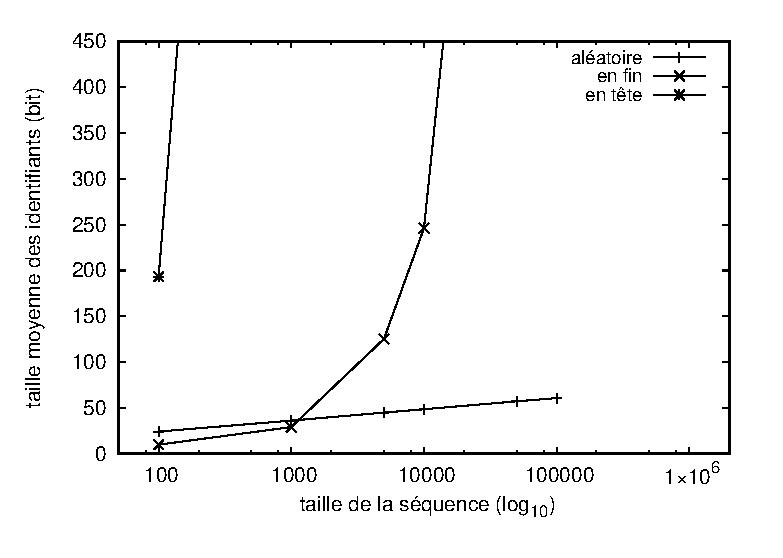
\includegraphics[width=0.8\textwidth]{img/lseq/logoot.eps}
    \caption[Mesures de référence de la taille des chemins]
    {\label{repl:img:logoot} Arbre à arité constante avec stratégie d'allocation
      adaptée à l'édition de gauche à droite. L'axe des abscisses montre la
      taille du document sur une échelle logarithmique en base décimale. L'axe
      des ordonnées montre la taille moyenne des chemins alloués.}
  \end{center}
\end{figure}


\paragraph{Objectif :} Fournir une référence aux futures expérimentations afin
de montrer les améliorations et les dégradations de chaque composant.

\paragraph{Description :} La simulation concerne trois documents artificiels
construits respectivement par un comportement d'édition aléatoire, un
comportement d'édition monotone de gauche à droite et un comportement d'édition
monotone de droite à gauche. La fonction d'allocation utilise un arbre d'arité
maximale constante et une seule sous-fonction d'allocation conçue pour l'édition
monotone de gauche à droite. Cette configuration correspond aux stratégies de
l'état de l'art~\cite{preguica2009commutative, weiss2009logoot}.  La moyenne de
la taille des identifiants est mesurée à 100, 1k, 5k, 10k, 50k, 100k insertions.

\paragraph{Résultat :} La figure~\ref{repl:img:logoot} montre les résultats de
cette expérimentation. Nous observons tout d'abord que la taille des
identifiants croît logarithmiquement dans le cas des éditions faites à des
positions aléatoires. Ensuite, les comportements d'édition monotone conduisent
tout deux à une croissance linéaire. Toutefois, l'édition de gauche à droite
reste bien plus efficace que l'édition de droite à gauche.

\paragraph{Explication :} Le comportement d'édition aléatoire conduit à une
structure d'arbre équilibrée. Les identifiants alloués restent petits. Le
comportement d'édition monotone de gauche à droite conduit à une croissance
linéaire mais relativement faible. En effet, la stratégie d'allocation employée
est conçue pour ce comportement : des branches sont laissées disponibles en vue
des prochaines insertions. La taille des identifiants grandit donc
lentement. Toutefois, comme l'arité maximale de l'arbre reste constante, la
structure ne s'adapte pas à la taille du document, d'où la croissance
linéaire. Dans le cas du comportement d'édition monotone de droite à gauche,
l'augmentation de la taille des identifiants est très forte car la stratégie
employée favorise le comportement d'édition opposé. Ainsi les insertions ont tôt
fait de ne plus avoir d'espace disponible conduisant à la création d'un nouvel
espace, i.e. la profondeur de l'arbre augmente. L'augmentation reste linéaire.

\subsection{Arbre exponentiel}

\begin{figure}
  \begin{center}
    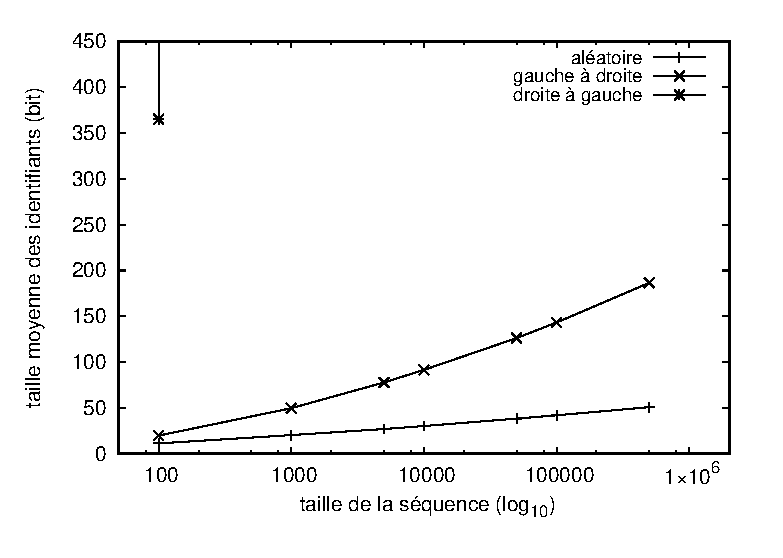
\includegraphics[width=0.8\textwidth]{img/lseq/double.eps}
    \caption[Influence de l'arbre exponentiel sur la taille des chemins]
    {\label{repl:img:exponentialtree} Arbre exponentiel avec stratégie
      d'allocation adaptée à l'édition de gauche à droite. L'axe des abscisses
      montre la taille du document sur une échelle logarithmique en base
      décimale. L'axe des ordonnées montre la taille moyenne des chemins
      alloués.}
  \end{center}
\end{figure}

\paragraph{Objectif :} Montrer que l'utilisation d'un arbre exponentiel permet
d'allouer des chemins dont la taille croît de manière polylogarithmique par rapport
au nombre d'insertions. Montrer que lorsque le comportement d'édition va à
l'encontre de celui prévu, les identifiants alloués ont une croissance
quadratique.

\paragraph{Description :} Trois documents sont créés artificiellement par
insertions successives de caractères. Pour chacun, un comportement d'édition
différent est simulé :
\begin{inparaenum}[(i)]
\item aléatoire,
\item monotone de gauche à droite et
\item monotone de droite à gauche.
\end{inparaenum}
La fonction d'allocation est conçue pour l'édition de gauche à droite et utilise
un arbre exponentiel.  La moyenne de la taille des identifiants est mesurée à
100, 1k, 5k, 10k, 50k, 100k, 500k insertions. 

\paragraph{Résultat :} La figure~\ref{repl:img:exponentialtree} montre les
résultats des mesures effectuées pendant la simulation. Nous observons qu'avec
un comportement d'édition aléatoire, et similairement aux mesures de références
(cf. figure~\ref{repl:img:logoot}), la croissance des identifiants est optimale
puisqu'elle suit un logarithme par rapport au nombre d'insertions dans le
document. Lors de l'édition monotone de gauche à droite, la croissance des
chemins est polylogarithmique par rapport au nombre d'insertions. En revanche,
l'édition de droite à gauche entraîne une augmentation quadratique de la taille
des identifiants.

\paragraph{Explication :} L'édition à des positions aléatoires place les
éléments au hasard dans la séquence. L'arbre est équilibré car nulle branche
n'est favorisée. À terme, les branches proches de la racine sont remplies
entièrement. Dans ce cas, les chemins sont de taille logarithmique ce qui
constitue la borne minimale. Lors du comportement d'édition monotone de gauche à
droite, les chemins les plus à gauche sont alloués réservant de l'espace aux
insertions futures. De plus, puisque l'arité de l'arbre double à chaque niveau,
il peut accueillir deux fois plus de chemins à un prix minime (1 bit additionnel
par niveau). Pour cette même raison, la croissance des identifiants devient
quadratique lors de l'édition de droite à gauche : quelques insertions suffisent
à faire augmenter la profondeur de l'arbre. L'arité maximale augmente alors
rapidement et le prix des identifiants explose. Dans ce cas, la taille des
chemins croît de manière quadratique.


\subsection{Sous-fonctions d'allocation}

\begin{figure}
  \begin{center}
    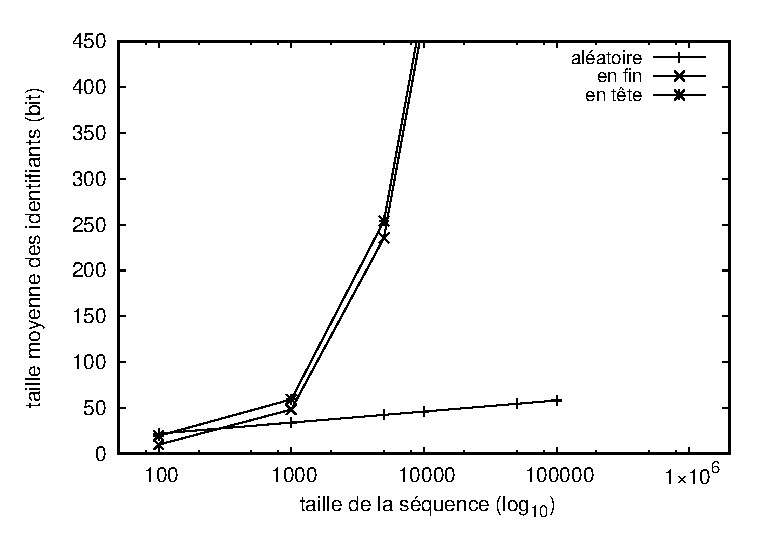
\includegraphics[width=0.8\textwidth]{img/lseq/robin.eps}
    \caption[Influence de deux sous-fonctions d'allocations sur la taille des
    chemins] {\label{repl:img:suballocation} Arbre à arité constante et deux
      sous-stratégies d'allocation. L'axe des abscisses montre la taille du
      document sur une échelle logarithmique en base décimale. L'axe des
      ordonnées montre la taille moyenne des chemins alloués.}
  \end{center}
\end{figure}

\paragraph{Objectif :} Montrer que deux sous-fonctions d'allocation conçues avec
des objectifs antagonistes et assignées à chaque profondeur de l'arbre
permettent de gèrer les comportements d'édition simples : monotones et
aléatoire. Montrer que la progression des identifiants reste linéaire par
rapport à la taille du document.

\paragraph{Description :} La simulation concerne trois documents grossissant au
rythme des opérations d'insertion effectuées respectivement de gauche à droite,
de droite à gauche et aléatoirement. La fonction d'allocation utilise un arbre
dont l'arité maximale est constante. De plus, chaque niveau se voit attribuer
une sous-fonction d'allocation, i.e., les niveaux pairs avec une fonction conçue
pour l'édition de gauche à droite et les niveaux impairs avec une fonction
adaptée à l'édition de droite à gauche. Nous mesurons la moyenne de la taille
des chemins composant les identifiants à 100, 1k, 5k, 10k, 50k, 100k insertions.

\paragraph{Résultat :} La figure~\ref{repl:img:suballocation} montre les
résultats obtenus à la suite de ces simulations. Nous observons tout d'abord que
les chemins restent logarithmiques sous un comportement d'édition
aléatoire. Nous observons aussi que, pour les deux types d'édition monotone, la
croissance est linéaire. De plus, les mesures sont quasiment identiques dans les
deux cas.

\paragraph{Explication :} Tout comme pour les expériences précédentes
(cf. figure~\ref{repl:img:logoot} et~\ref{repl:img:exponentialtree}), l'édition
à des positions aléatoires à pour effet d'équilibrer l'arbre représentant le
document répliqué. Les chemins résultant de ce comportement grandissent de
manière logarithmique. Grâce à une alternance des sous-fonctions d'allocation,
la taille des chemins alloués lors des comportements d'édition monotone augmente
lentement. Malgré tout, la progression reste linéaire. De plus, elle augmente
deux fois plus rapidement que sans cette alternance avec un comportement
d'édition favorable (cf. figure~\ref{repl:img:logoot}). En effet, dans le cas de
ces simulations, un niveau sur deux est perdu car consommé trop vite : la
sous-fonction d'allocation assignée à ce niveau n'était pas celle conçue pour le
comportement d'édition courant.


\subsection{Arbre exponentiel et sous-fonctions}

\begin{figure}
  \begin{center}
    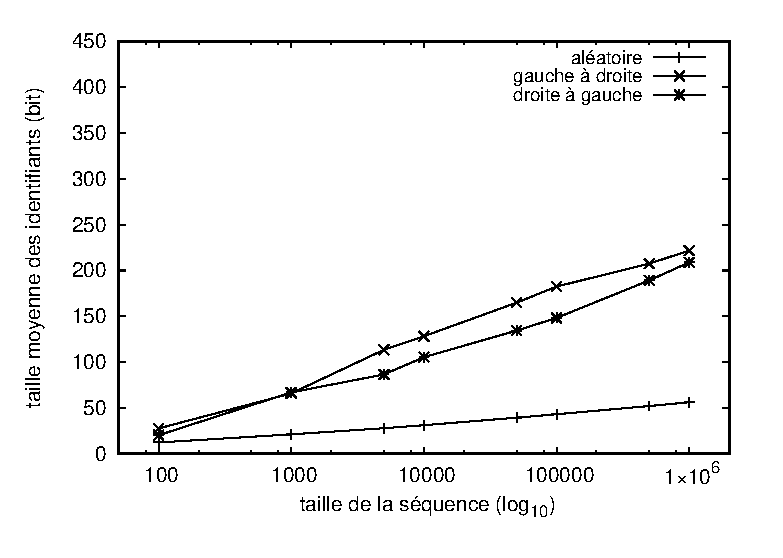
\includegraphics[width=0.8\textwidth]{img/lseq/lseq.eps}
    \caption[Combinaison de l'arbre exponentiel et des sous-fonctions
    d'allocation] {\label{repl:img:lseq} Arbre exponentiel avec deux
      sous-stratégies d'allocation. L'axe des abscisses montre la taille du
      document sur une échelle logarithmique en base décimale. L'axe des
      ordonnées montre la taille moyenne des chemins alloués.}
  \end{center}
\end{figure}

\paragraph{Objectif :} Montrer que l'utilisation combinée d'un arbre exponentiel
et de sous-fonctions d'allocation permet de pallier leurs faiblesses respectives
et d'obtenir une stratégie d'allocation sous-linéaire par rapport au nombre
d'insertions effectuées dans le document.

\paragraph{Description :} Trois documents chacun édité d'une façon différente :
l'auteur du premier possède un comportement d'édition aléatoire; l'auteur du
second possède un comportement d'édition monotone de gauche à droite; l'auteur
du troisième de droite à gauche. La fonction d'allocation utilise un arbre
exponentiel et deux sous-fonctions d'allocation conçues pour gérer les éditions
monotones. Les sous-fonctions d'allocation sont assignées aléatoirement à chaque
niveau de l'arbre. Les mesures sont faites à 100, 1k, 5k, 10k, 50k, 100k, 500k,
1M insertions.

\paragraph{Résultat :} La figure~\ref{repl:img:lseq} affiche les résultats
obtenus lors de cette expérimentation. Nous observons que la progression de la
taille des identifiants lors du comportement d'édition aléatoire reste
logarithmique. Lors des deux autres comportements d'édition monotone, la
croissance des identifiants suit une progression polylogarithmique par rapport au
nombre d'insertions effectuées dans la séquence. Cette observation confirme
l'analyse en complexité spatiale des identifiants
(cf. §\ref{repl:subsec:space}). Cependant, nous observons de petites
différences entre les deux courbes résultant des comportements d'édition monotone.

\paragraph{Explication :} Le comportement d'édition aléatoire conduit à un arbre
exponentiel équilibré, d'où la croissance logarithmique des identifiants. Les
autres cas d'édition sont très similaires car les sous-fonctions d'allocation
ont la même probabilité d'apparaître. Les différences s'expliquent par les
différents choix lors des exécutions. La progression sous-linéaire s'explique
grâce à l'augmentation d'arité de l'arbre lorsqu'il gagne en profondeur, i.e.,
chaque nœud de l'arbre peut posséder jusqu'à deux fois plus de fils que son
parent. Lorsque la sous-fonction d'allocation employée ne s'accorde pas avec le
comportement d'édition, la profondeur de l'arbre est incrémentée
rapidement. Lorsque finalement la bonne sous-fonction d'allocation est trouvée,
celle-ci couvre les dépenses qu'il a fallu déployer pour la trouver, i.e., la
perte de niveaux dans l'arbre.

\subsection{Complexité spatiale}

\subsubsection{Traces réelles}

\begin{figure*}
  \centering
  \subfloat[Document Wikipédia principalement édité de gauche à droite]
  [\label{repl:img:motivationsA}Document Wikipédia de très grande
  taille principalement édité de gauche à droite.]
  {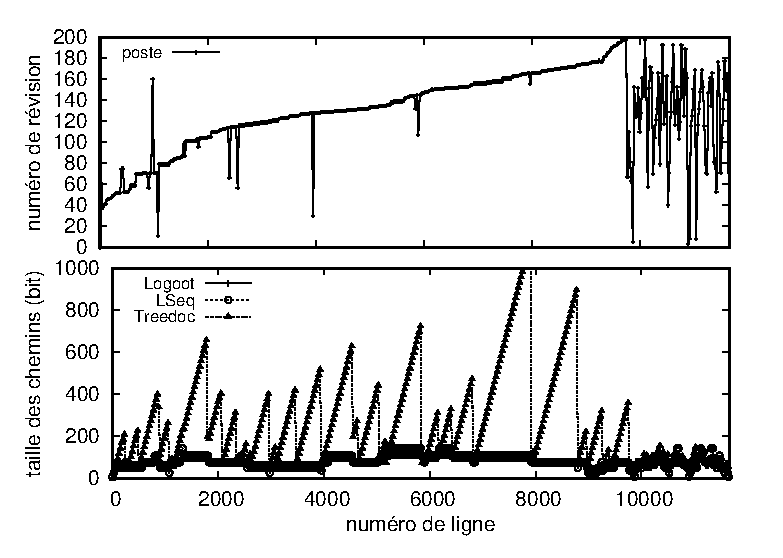
\includegraphics[width=0.8\textwidth]{img/lseq/poste.eps}}
  \hspace{10pt}
  \subfloat[Document Wikipédia principalement édité de droite à gauche]
  [\label{repl:img:motivationsB}Document Wikipédia de petite taille
  principalement édité de droite à gauche.]
  {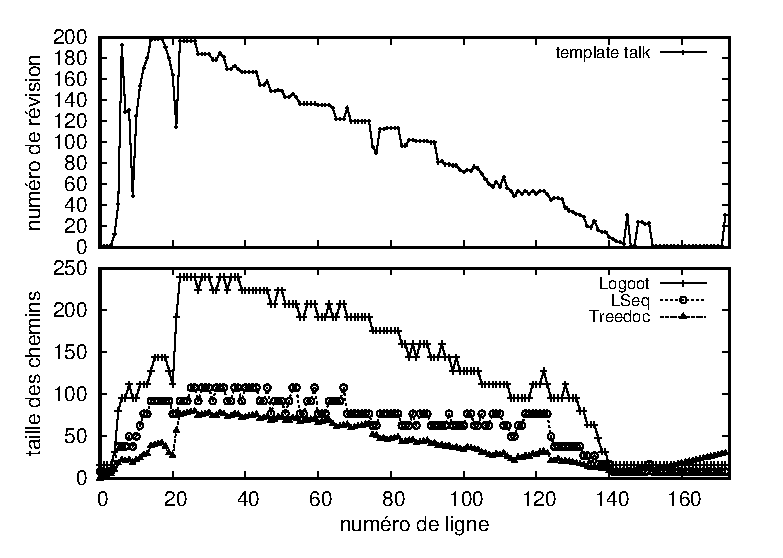
\includegraphics[width=0.8\textwidth]{img/lseq/templatetalk.eps}}
  \caption[Taille du chemin alloué pour chaque ligne dans Wikipédia]
  {\label{repl:img:motivations} Taille du chemin alloué pour chaque ligne du
    document. L'axe des abscisses montre le numéro de la ligne concernée. L'axe
    des ordonnées de la partie haute de la figure montre l'âge de la
    ligne. L'axe des ordonnées de la partie basse de la figure montre la taille
    binaire du chemin alloué.}
\end{figure*}

L'encyclopédie Wikipédia~\cite{wikipedia} répertorie des millions d'articles
écrits collaborativement. Un utilisateur peut lire un article et, s'il le
souhaite, en modifier le contenu. Lorsque ses modifications sont achevées, il
les soumet à Wikipédia. Deux issues possibles :
\begin{inparaenum}[(i)]
\item La contribution est acceptée et sera visible de tous ou
\item la contribution est rejetée car un autre utilisateur a effectué une
  modification en concurrence et l'a soumise en premier. Il faut alors réviser
  la version rejetée afin de l'adapter à la version la plus à jour avant de la
  soumettre à nouveau, si nécessaire.
\end{inparaenum}
Wikipédia garde l'historique des modifications apportées à tous les articles
depuis leur création. Nous sommes alors à même de rejouer les éditions --
nommées révisions -- dans l'ordre où elles ont été effectuées. Toutefois, toute
trace de concurrence est effacée par le protocole d'édition même. D'autre part,
la granularité est fixée à la ligne et non au caractère. En cela, les
simulations sur corpus Wikipédia diffèrent légèrement de la réalité.


\paragraph{Objectif :} Montrer que ni Logoot ni Treedoc ne parviennent à fournir
des identifiants dont la taille soit satisfaisante quel que soit le document
créé grâce à des traces réelles. En revanche, \LSEQ y parvient.

\paragraph{Description :} Logoot est configuré avec une arité maximale de
$2^{16}$. \LSEQ est configuré avec arité maximale de départ de $2^{8}$. Treedoc
a une arité de $2^1$ et est configuré pour utiliser sa méthode originelle peu
adaptée à l'édition monotone -- son autre stratégie étant équivalente à la
stratégie de Logoot. Les documents considérés sont des articles extraits de
Wikipédia et rejoués sur 200 révisions. L'un des articles atteint jusqu'à 10k
lignes principalement ajoutées de gauche à
droite\footnote{\scriptsize\url{https://fr.wikipedia.org/wiki/Liste_des_bureaux_de_poste_français_classés_par_oblitération_Petits_Chiffres}}. L'autre
article atteint seulement 200 lignes mais est principalement édité de droite à
gauche\footnote{\scriptsize\url{https://en.wikipedia.org/wiki/Template_talk:Did_you_know}}.

\paragraph{Résultat :} Les figures~\ref{repl:img:motivationsA}
et~\ref{repl:img:motivationsB} montrent la taille de l'identifiant associé à
chaque ligne. Nous observons que Treedoc possède des chemins qui augmentent très
vite quel que soit le type d'édition. Lorsque le nombre d'insertions successives
est très grand (cf. figure~\ref{repl:img:motivationsA}) les chemins atteignent
des tailles très élevées avec une claire croissance linéaire. Dans ce cas,
Logoot se comporte mieux. Bien que \LSEQ démarre avec une base plus faible il
présente des résultats équivalents à Logoot. En revanche, dans le cadre de
l'édition de droite à gauche (cf. figure~\ref{repl:img:motivationsB}), Logoot
alloue des chemins dont la taille augmente extrêmement rapidement. Treedoc se
comporte de manière similaire bien que les valeurs mesurées soient plus
faibles. Les identifiants alloués par \LSEQ se stabilisent.

%% Pour retrouvrer de bonnes performances, l'exécution d'un protocole de
%% relocalisation des chemins devient nécessaire.

\paragraph{Explication :} Dans les deux types d'édition, Treedoc et Logoot
allouent des identifiants dont la complexité est linéaire. Ainsi, plus les
insertions se succèdent, plus l'arbre est déséquilibré, plus la taille du chemin
augmente. Cependant, comme Treedoc alloue des chemins où chaque pas est binaire
($\mathcal{P}\in \mathbb{N}_{<2}.\mathbb{N}_{<2}\ldots\mathbb{N}_{<2}$), les
chemins restent plus petits que ceux de Logoot dans le cadre du document édité
de droite à gauche. D'un autre côté, Logoot a conçu sa stratégie pour l'édition
de gauche à droite. Dès lors, si le comportement suit cette hypothèse, les
identifiants grossissent par palier -- linéairement certes, mais
lentement. \LSEQ ne favorise aucun comportement d'édition et adapte la taille de
ses identifiants à la taille du document. Ainsi, les deux types de document
sont gérés : beaucoup d'insertions effectuées de gauche à droite; peu
d'insertions effectuées de droite à gauche.


\subsubsection{Documents synthétiques}

\begin{figure}
  \begin{center}
    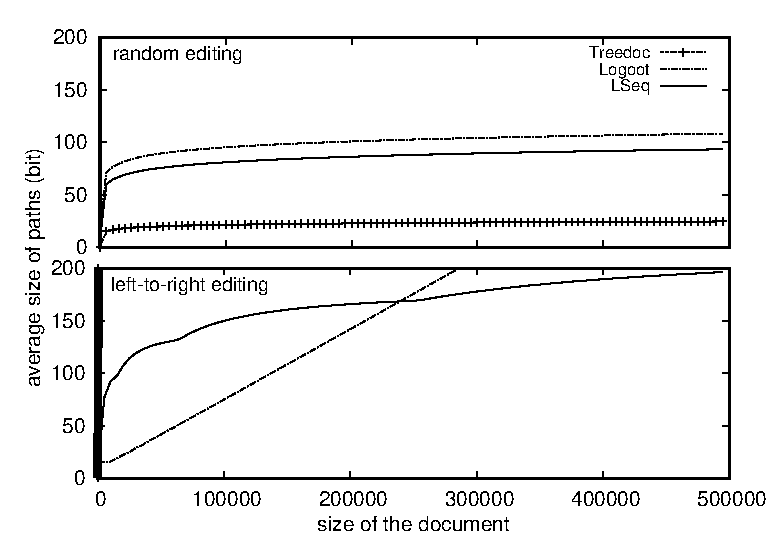
\includegraphics[width=0.8\textwidth]{img/lseq/space.eps}
    \caption[Taille moyenne des chemins sur des documents synthétiques]
    {\label{repl:img:motivationartificial}Taille moyenne des chemins alloués en
      fonction du nombre d'insertions successives dans la séquence. L'axe des
      abscisses montre le nombre d'insertions dans la séquence. L'axe des
      ordonnées montre la taille moyenne de la représentation binaire des
      chemins alloués.}
  \end{center}
\end{figure}

\paragraph{Objectif :} Montrer la progression de la taille des identifiants
alloués par les fonctions d'allocation Logoot, \LSEQ et Treedoc sur des
documents synthétiques.

\paragraph{Description :} Deux types de document synthétique sont créés. Tout
d'abord, un premier document est créé grâce à des insertions à des positions
aléatoires dans la séquence. Le second document est créé grâce à des insertions
successives en fin de document. La fonction d'allocation des chemins de Logoot
est spécifiquement conçue pour gérer ce dernier type d'édition. Logoot est
configuré avec une arité maximale de $2^{16}$, \LSEQ est configuré avec une
arité maximale de départ de $2^8$, Treedoc a une arité maximale de $2^1$.  La
taille moyenne des chemins composant les identifiants est mesurée à chaque
nouvelle insertion. Le document atteint 500k caractères.

\paragraph{Résultat :} La figure~\ref{repl:img:motivationartificial} montre les
résultats de cette simulation. La partie du haut montre les résultats du
document édité à des positions aléatoires. La partie du bas montre les résultats
du document édité à la fin. Nous observons que l'édition à des positions
aléatoires entraîne une génération de chemins dont la taille est logarithmique,
que ce soit pour Logoot, \LSEQ ou Treedoc. Dans ce cas, Treedoc est meilleur que
Logoot et \LSEQ. Nous observons aussi que l'édition de gauche à droite entraine
une croissance extrêmement rapide pour les identifiants alloués par Treedoc (la
courbe est superposée à l'axe des ordonnées). De son côté, Logoot alloue des
chemins dont la taille augmente moins rapidement. Malgré cela, la croissance
reste linéaire par rapport au nombre d'insertions dans la séquence. À terme,
l'exécution d'un protocole de relocalisation des chemins devient nécessaire pour
retrouver de bonnes performances. En revanche, \LSEQ alloue des identifiants
dont la croissance est sous-linéaire par rapport au nombre d'insertions. À terme,
l'allocation de \LSEQ finit par surpasser celle de l'état de l'art.

\paragraph{Explication :} Les fonctions d'allocation Logoot, \LSEQ et Treedoc
utilisent une structure d'arbre pour allouer le chemin associé à chaque
caractère. Dans le cadre de l'édition aléatoire, l'arbre reste équilibré au
cours des insertions. Les branches les plus basses se remplissent au maximum de
leur capacité. Par conséquent, les identifiants alloués par ces trois approches
croissent logarithmiquement par rapport au nombre d'insertions. L'arité de
l'arbre de Treedoc étant inférieure à l'arité de l'arbre de Logoot et \LSEQ,
Treedoc propose de meilleurs identifiants. Dans le cadre de l'édition de gauche
à droite, chaque nouvelle insertion dans Treedoc ajoute un bit au chemin
généré. La croissance est linéaire par rapport au nombre d'insertions dans la
séquence.
% et extrêmement rapide.
La fonction d'allocation de Logoot est conçue pour gérer ce type
d'édition. Chaque niveau de l'arbre possède une branche remplie
d'éléments. Toutefois, le nombre d'éléments accueillis par chaque branche reste
constant, d'où la croissance linéaire de la taille des chemins générés. Avec
\LSEQ, l'arbre est exponentiel : chaque nœud de l'arbre possède une arité
maximale deux fois supérieure à son parent. Ainsi, plus elles sont profondes,
plus les branches peuvent accueillir d'éléments. Par conséquent, la vitesse
d'augmentation de profondeur de l'arbre exponentiel diminue lorsque le nombre
d'insertions augmente.


\subsection{Complexité temporelle}

\begin{figure}
  \begin{center}
    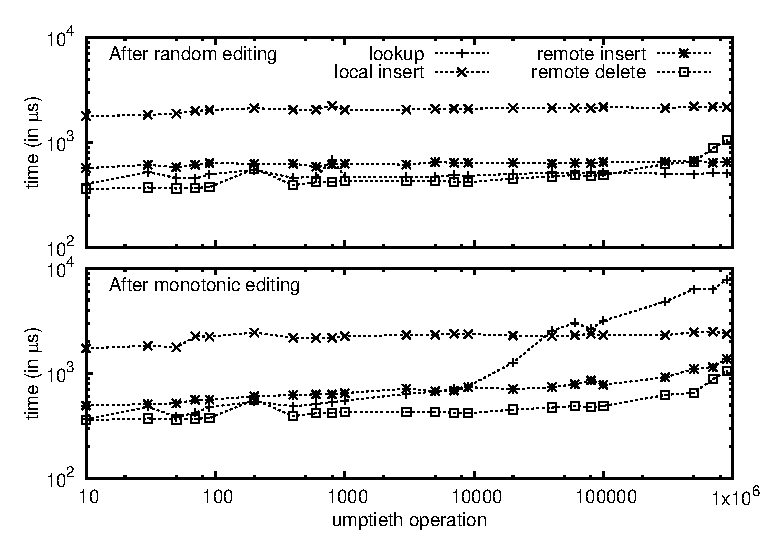
\includegraphics[width=0.8\textwidth]{img/lseq/time.eps}
    \caption[Performances de \LSEQ] {\label{repl:img:time} Performances de la
      énième opération effectuée sur \LSEQ. L'axe des abscisses montre le numéro
      de la énième opération. L'axe des ordonnées montre le temps d'exécution de
      l'opération en microsecondes. La figure du haut considère une structure
      remplie par des insertions aléatoires. La figure du bas considère une
      structure remplie par insertions monotones.}
  \end{center}
\end{figure}

\paragraph{Objectif :} Confirmer l'analyse en complexité temporelle de
\LSEQ. Des performances passant à l'échelle sont attendues.

\paragraph{Description :} Cette expérience implique un utilisateur artificiel
unique effectuant des opérations sur sa réplique du document. Le banc d'essai
s'est déroulé sur un \emph{MacBook Pro} comportant un processeur \emph{2.5 GHz
  Intel Core i5}, la version 4.1.1 de \emph{Node.js}, sur une architecture
Darwin 64-bit. Pour chaque opération, un document de $I-1$ caractères est créé
artificiellement. Les mesures s'effectuent sur la $I$\up{ème} opération. Les
opérations prises en compte sont la fonction \textsc{lookup}, la partie locale
de l'insertion, la partie distante de l'insertion, et la partie distante de la
suppression -- la partie locale de cette dernière ne comprend que la propagation
de l'identifiant ciblé aux autres membres. Les mesures sont effectuées à
plusieurs reprises sur deux types de document. Tout d'abord, un document généré
par un comportement d'édition aléatoire, i.e., l'arbre \LSEQ est
équilibré. Ensuite, un document généré par un comportement d'édition monotone,
i.e., une seule branche de l'arbre \LSEQ est remplie. 
%Nous nous intéressons aux
%tendances plutôt qu'aux valeurs absolues. En effet, 
Le langage JavaScript opère de nombreuses optimisations à la volée. Afin
de montrer la contribution réelle de chacune des opérations, ces optimisations
ont été limitées au maximum. Les performances réelles des opérations sont donc
nettement meilleures que celles présentes dans cette expérimentation.

\paragraph{Résultat :} La figure~\ref{repl:img:time} montre les résultats de
cette expérimentation. Nous observons que les valeurs mesurées, dans le cadre
d'un arbre remplies par des éditions aléatoires, ne croissent pratiquement pas
et ce quelle que soit l'opération. D'un autre côté, lorsque l'insertion locale
après édition monotone reste stable, nous observons une croissance linéaire du
temps d'exécution de la fonction \textsc{lookup} et une plus faible évolution
pour les parties distantes des opérations d'insertion et de suppression.

\paragraph{Explication :} Après un comportement d'édition aléatoire, l'arbre de
\LSEQ est équilibré. Par conséquent l'influence d'une opération se limite à un
petit sous ensemble d'éléments composant le document. Par exemple, la fonction
\textsc{lookup} n'a pas besoin d'explorer chaque élément de l'arbre. Elle rejette
rapidement de nombreuses branches sans importance à chaque niveau de l'arbre
car l'indice recherché ne tombe pas dans leur intervalle. Toutefois, cette
remarque n'est pas vraie en ce qui concerne un arbre rempli par un comportement
d'édition monotone. En effet, dans ce cas, la plupart des éléments sont
localisés dans l'une -- et la plus profonde -- des branches de l'arbre. Ainsi,
la fonction \textsc{lookup} va probablement explorer tous les niveaux et
inspecter chaque élément pour en compter le nombre de fils afin d'actualiser son
indice de progression courant. Les mesures concernant les opérations distantes
suivent le même raisonnement. Elles sont plus efficaces car l'exploration des
niveaux utilise la recherche dichotomique.


\subsection{Concurrence}

\begin{figure}
  \begin{center}
    \includegraphics[angle=-90,width=0.8\textwidth]{img/lseq/latency.eps}
    \vspace{25pt}
    \caption[Effet de la concurrence sur les identifiants]
    {\label{repl:img:latency}Effets de la concurrence sur la taille des
      identifiants. L'axe des abscisses montre le nombre d'insertions effectuées
      dans le document. L'axe des ordonnées montre la taille des messages envoyés
      (en octets).}
  \end{center}
\end{figure}

\paragraph{Objectif :} Montrer que plus la concurrence est élevée, plus les
identifiants alloués sont petits.

\paragraph{Description :} Deux utilisateurs artificiels dont le comportement est
monotone écrivent de gauche à droite un même document. Grâce à
netem~\cite{netem}, une latence est ajoutée sur le transport des messages créant
des opérations concurrentes. Les documents atteignent 10k caractères. Les
mesures sur la taille moyenne des messages envoyés sont effectuées tout au long
de l'expérimentation. La fonction d'allocation employée est celle de \LSEQ : un
arbre exponentiel avec deux sous-fonctions d'allocation.

\paragraph{Résultat :} La figure~\ref{repl:img:latency} montre les résultats de
cette expérimentation. Comme attendu, plus la latence est élevée, plus la
concurrence est élevée, plus les messages sont de petite taille. Les
expérimentations sans concurrence présentent donc la borne supérieure des
fonctions d'allocation. La figure~\ref{repl:img:latency} nous montre aussi, avec
une plus fine granularité, la croissance polylogarithmique de la taille des
messages qui confirme une seconde fois l'analyse en complexité spatiale des
identifiants.

\paragraph{Explication :} Les insertions effectuées par les participants ciblent
une même position dans le document. Toutefois, ils ne prennent connaissance de
cela que quelque temps plus tard, lorsque le message correspondant leur est
parvenu. Ainsi, les opérations sont réellement concurrentes. Les insertions
étant effectuées en concurrence à la même position dans la séquence, les
opérations partagent le même espace d'allocation. Les identifiants ont une
chance d'obtenir le même chemin dans l'arbre. En moyenne, ils sont plus
rapprochés les uns des autres. Il est important de noter que les documents
résultant de ces expérimentations sont différents. En d'autres termes, la série
de caractères composant le document est différente en fonction de la latence.


%%% Local Variables:
%%% mode: latex
%%% TeX-master: "../../paper"
%%% End:
